\documentclass[12pt, twoside]{article}
\documentclass[12pt, twoside]{article}
\usepackage[letterpaper, margin=1in, headsep=0.2in]{geometry}
\setlength{\headheight}{0.6in}
%\usepackage[english]{babel}
\usepackage[utf8]{inputenc}
\usepackage{microtype}
\usepackage{amsmath}
\usepackage{amssymb}
%\usepackage{amsfonts}
\usepackage{siunitx} %units in math. eg 20\milli\meter
\usepackage{yhmath} % for arcs, overparenth command
\usepackage{tikz} %graphics
\usetikzlibrary{quotes, angles}
\usepackage{graphicx} %consider setting \graphicspath{{images/}}
\usepackage{parskip} %no paragraph indent
\usepackage{enumitem}
\usepackage{multicol}
\usepackage{venndiagram}

\usepackage{fancyhdr}
\pagestyle{fancy}
\fancyhf{}
\renewcommand{\headrulewidth}{0pt} % disable the underline of the header
\raggedbottom
\hfuzz=2mm %suppresses overfull box warnings

\usepackage{hyperref}
\usepackage{float}

\title{Algebra 2}
\author{Chris Huson}
\date{October 2024}

\fancyhead[LE]{\thepage}
\fancyhead[RO]{\thepage \\ First and last name: \hspace{2.5cm} \,\\ Section: \hspace{2.5cm} \,}
\fancyhead[LO]{BECA / Huson / Algebra 2: Polynomials \\* 24 October 2024}

\begin{document}

\subsubsection*{2.19 Test: Polynomials}
\begin{enumerate}

\subsubsection*{A1-A.APR.1 Add, subtract, and multiply polynomials}
\item Evaluate each polynomial for the given value of $x$.
\begin{multicols}{2}
    \begin{enumerate}[itemsep=1cm]
        \item $f(x)=2x^3-x^2-5x+9$\\[0.25cm] 
        $f(0) = $
        \item $g(x)=4x^2+x-7$ \\[0.25cm] 
        $g(1) = $
    \end{enumerate}
    \end{multicols} \vspace{1cm}

\item Write the sum in standard form $(x^3+12x^2-7x+3)+(2x^3-3x^2-2x-6)$. \vspace{5cm}

\item Find the difference $f(x)-g(x)$ as a polynomial in standard form, with \\[0.25cm]
    $f(x)=x^3-2x^2+3x+5$ and $g(x)=x^2-2x-5$. \vspace{5cm}


\item Select the expression that is equivalent to $x^2-7x+10$.
    \begin{multicols}{2}
    \begin{enumerate}
        \item $(x-2)(x-5)$
        \item $(x+2)(x+5)$
        \item $(x-2)(x+5)$
        \item $(x+2)(x-5)$
    \end{enumerate} 
    \end{multicols}

\newpage
\subsubsection*{A1-A.APR.3 Identify zeros of polynomials when factorizations are available.}
\item Write down the solutions to the equation $-2x(x+5)(x-9)(2x+1)=0$. \vspace{2cm}
    
\item The polynomial $p$ is a function of $x$. The graph of $p$ has zeros at $-4$, $-\frac{2}{3}$, $0$ and $9$. Select $\bf{all}$ the expressions that could represent $p$. \vspace{0.25cm}
    \begin{multicols}{2}
    \begin{enumerate}
        \item $3x(x-4)(x+\frac{2}{3})(x+9)$
        \item $-x(x+4)(x+\frac{2}{3})(x-9)$
        \item $-3x(x+4)(3x+2)(x-9)$
        \item $3x(x+4)(2x-3)(x-9)$
        \item $-3x(x+4)(3x+2)(x-9)^2$
        \item $x(x+4)(x+\frac{2}{3})(x-9)^2$
    \end{enumerate}
    \end{multicols}
        \vspace{0.25cm}

\item Which expression is equivalent to $2(3x+4)(x-1)(x-3)$? \vspace{0.25cm}
    \begin{enumerate}
        \item $6x^3-16x^2-14x+24$ 
        \item $6x^3-4x^2-34x-24$ 
        \item $3x^3-8x^2-7x+12$ 
        \item $6x^3+20x^2-2x-24$ 
    \end{enumerate} \vspace{0.25cm}

\item Let $f$ be a polynomial function of $x$ where $f(x)=2x^3+5x^2-28x-15$. If $x-3$ is a factor of $f$, write an equation for $f$ as a product of linear factors.
\vspace{5cm}

\newpage
\item Let $P$ be a polynomial function of $x$, and $P(x)=x^4-dx^3+8x^2-14x+16$. If $x-2$ is a factor of the polynomial, what is the value of $d$? Explain or show how you know.
\vspace{5cm}

\subsubsection*{A2-F.IF.7c Graph polynomials, identify zeros, end behavior}
\item Here is the graph of a quadratic function. Which of the following could be its equation?
\begin{multicols}{2}
    \begin{enumerate}
        \item $y=(x+2)(x-4)$
        \item $y=(x-2)(x+4)$
        \item $y=(x+2)(x+4)$
        \item $y=(x-2)(x-4)$
    \end{enumerate}% \vspace{1cm} \;

    \columnbreak
    \begin{tikzpicture}[xscale=0.7, yscale=0.2]
        \draw [thick, ->] (-4.2,0) -- (5.4,0) node [above] {$x$};
        \draw [thick, ->] (0,-9.2)--(0,8.5) node [right] {$y$};
        \foreach \x in {-4,...,-1,1,2,...,5} \draw (\x cm,10pt)--(\x cm,-10pt) node[below] {$\x$};
        \draw [thick, <->,smooth,samples=20,domain=-3:5] plot(\x,\x*\x-2*\x-8);
    \end{tikzpicture}
    \end{multicols}

\item Let $j(x)=-2(3x+4)(x-1)(x-3)^2$ be a polynomial function. 
    \begin{center}
    \begin{tikzpicture}[xscale=0.7, yscale=0.5]
        \draw [thick, ->] (-7.2,0) -- (7.5,0) node [above] {$x$};
        \draw [thick, ->] (0,-6.2)--(0,6.5) node [right] {$y$};
        \foreach \x in {-7,...,7} \draw (\x cm,5pt) -- (\x cm,-5pt);
    \end{tikzpicture}
    \end{center}
    \begin{enumerate}
        \item Sketch a graph of the function.
        \item Name all horizontal and vertical intercepts of the graph.
        \item State the end behavior of $j$.
    \end{enumerate}
        
\newpage
\subsubsection*{A2-F.BF.2 Write arithmetic and geometric sequences with recursive formulas}
\item Write a recursive formula for each sequence. Use subscript notation.
    \begin{multicols}{2}
    \begin{enumerate}
        \item $1, 2, 4, 8, 16, \dots$
        \item $\displaystyle \frac{1}{3}, \frac{2}{9}, \frac{8}{27}, \frac{16}{81},  \dots$ 
    \end{enumerate}
    \end{multicols} \vspace{4cm}

\item Write a recursive definition of the arithmetic sequence $a$. \\[0.5cm]
\renewcommand{\arraystretch}{1.5}
\begin{tabular}{|c|c|}
\hline
$n$ & $a_n$ \\
\hline
$1$ & $5$ \\
$2$ & $-5$ \\
$3$ & $-15$ \\
\hline
\end{tabular} \vspace{1cm}

\subsubsection*{6.EE.b: Solve one-variable equations}
\item Use the function $f(x) = \frac{1}{2}x-9$ to answer the questions.
    \begin{multicols}{2}
    \begin{enumerate}[itemsep=2cm]
        \item What is $f(0)$?
        \item Find $f(6)$
        \item Solve for $x$ if $f(x) = -2$.
    \end{enumerate}
    \end{multicols} \vspace{3cm}

\item Fill in the blank. The beginning of a new marking period is a good time to\\[0.5cm] 
``Turn over a new \underline{\hspace{2cm}}.''

\end{enumerate}
\end{document}